\chapter{Results and Discussion}
This chapter is dedicated to presenting and discussing the results generated by the system. 

\section{Results}
The project had various critical phases that were completed. The following phases and their results have been documented below.

\subsection{System Design Results}
The data capture system was designed to meet the specifications outlined in the methodology chapter. The device was comfortable, light weight and adjustable such that it could easily be used by a large variety of people. The device was also sturdy and well constructed allowing for long term usage. Pictured below is a subject wearing the data capture system.

\begin{figure}[!ht] 
\captionsetup{width=0.5\linewidth, font=small}  
\includegraphics[width=0.5\linewidth]{figures/pat_harness.png}
\caption{subject wearing the motion capture system }
\label{fig:pat_harness}
\end{figure}

The stereo housings were fully functional and offered a good fit for both the camera and the mounting hardware. Although the cameras moved during running they captured all the critical points in every single frame. The device in no way affected the gait of the subject as the system had a minimal footprint.



\subsection{Captured and Processed Data}
The system was fully capable of capturing all the data necessary to quantify the gait of a runner. 

The following is a graph of the accelerometer in the z-body frame against time.

From this graph it it the rhythmic motion of running is easy to see. a spike of close to 4g seen at the moment of impact and a maximum acceleration of around 1 g as the subject reaches maximum height.

\begin{figure}[!ht] 
\captionsetup{width=0.8\linewidth, font=small}  
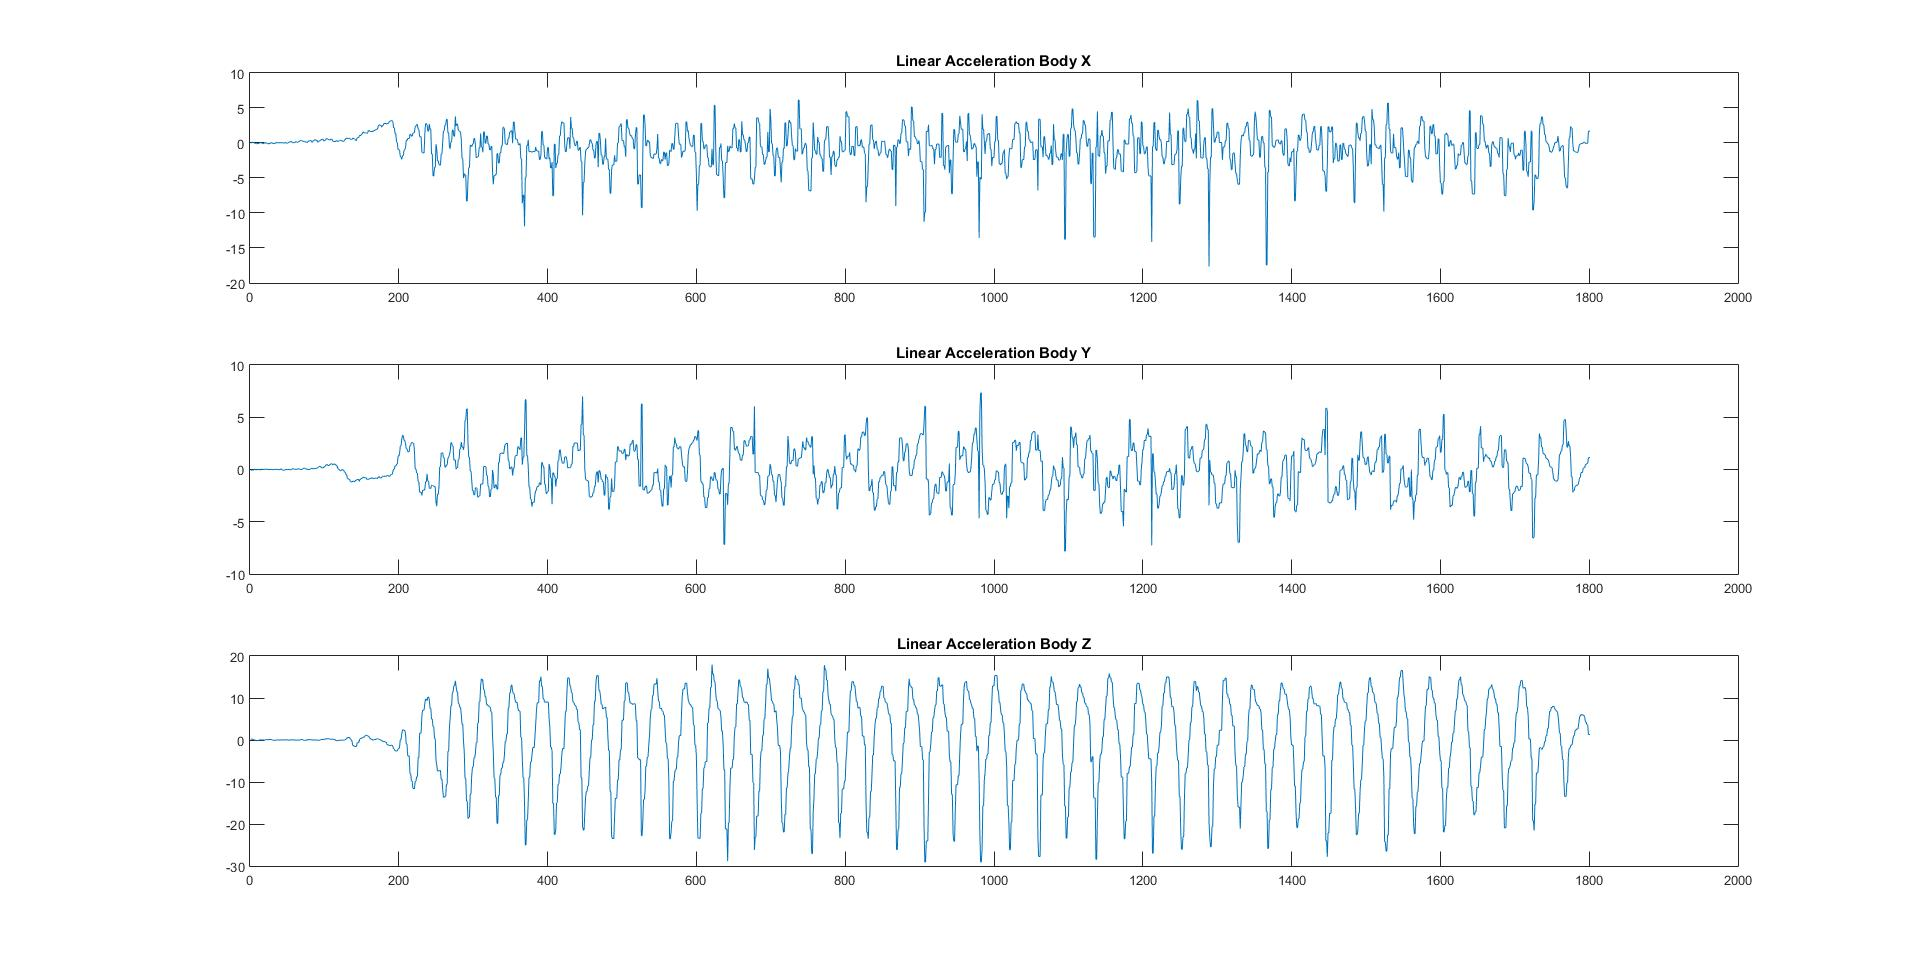
\includegraphics[width=0.5\linewidth]{figures/accelerometer.jpg}
\caption{iamge processing things}
\label{fig:accelerometer}
\end{figure}

gyroscope

\begin{figure}[!ht] 
\captionsetup{width=0.8\linewidth, font=small}  
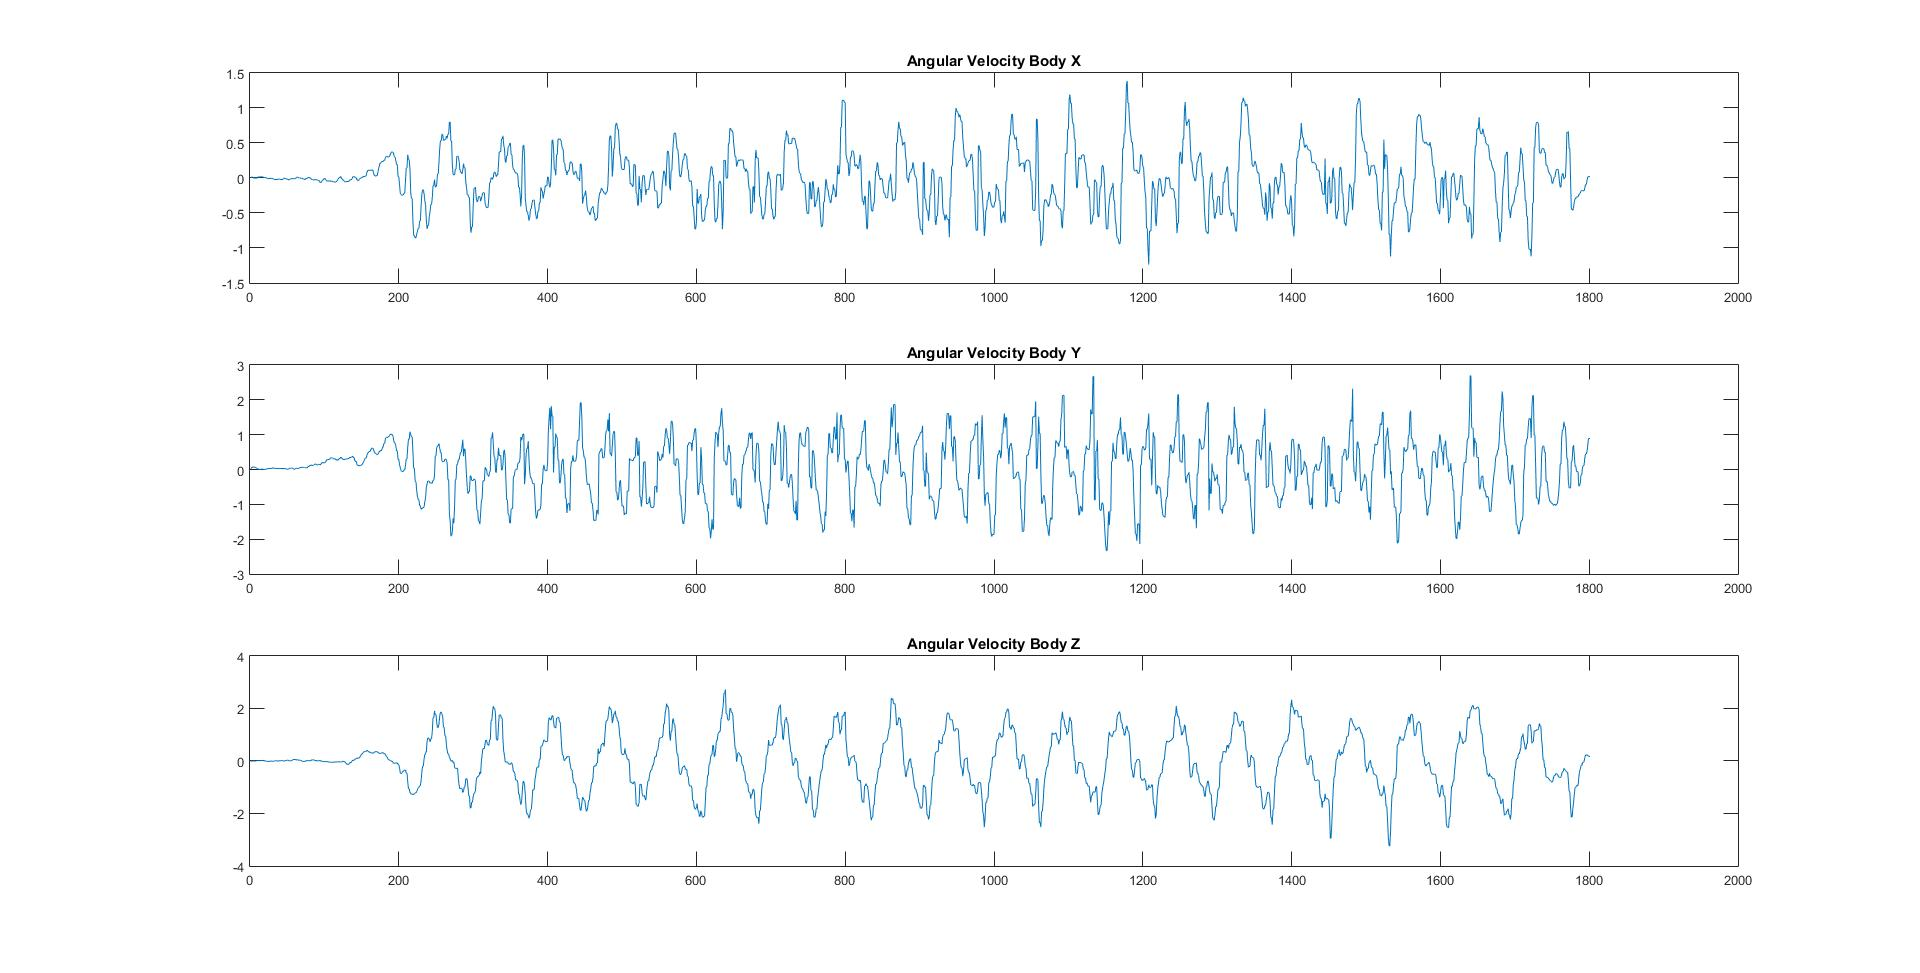
\includegraphics[width=0.5\linewidth]{figures/gyroscope.jpg}
\caption{iamge processing things}
\label{fig:gyroscope}
\end{figure}

magnetometer

\begin{figure}[!ht] 
\captionsetup{width=0.8\linewidth, font=small}  
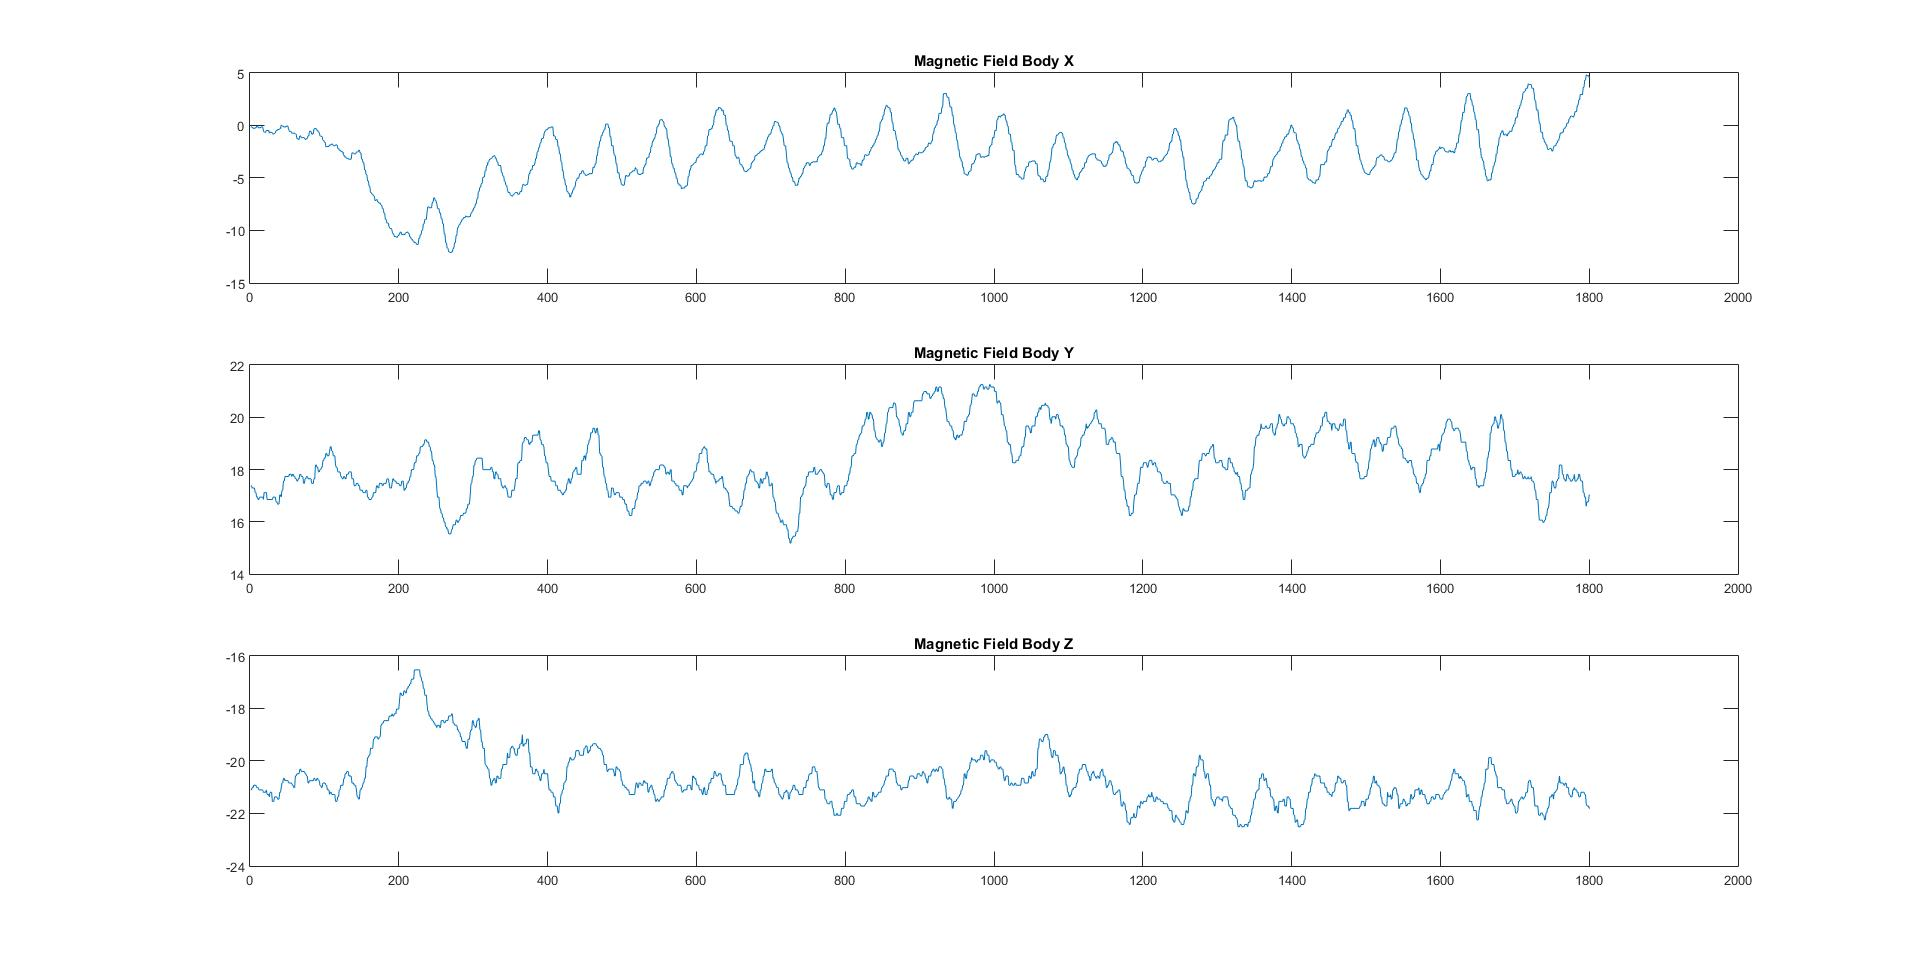
\includegraphics[width=0.5\linewidth]{figures/magnetometer.jpg}
\caption{iamge processing things}
\label{fig:magnetometer}
\end{figure}

gps and barometer

\begin{figure}[!ht] 
\captionsetup{width=0.8\linewidth, font=small}  
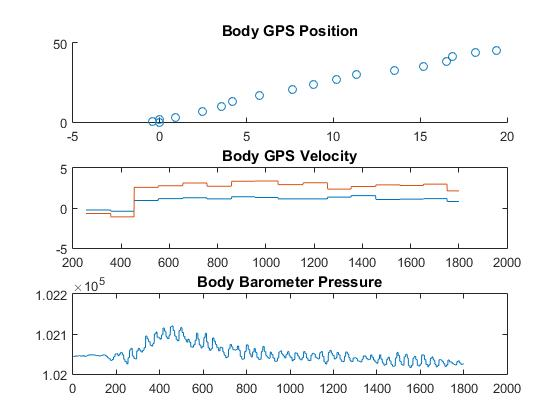
\includegraphics[width=0.5\linewidth]{figures/gps.jpg}
\caption{iamge processing things}
\label{fig:gps}
\end{figure}





Image Processing graph

\begin{figure}[!ht] 
\captionsetup{width=0.8\linewidth, font=small}  
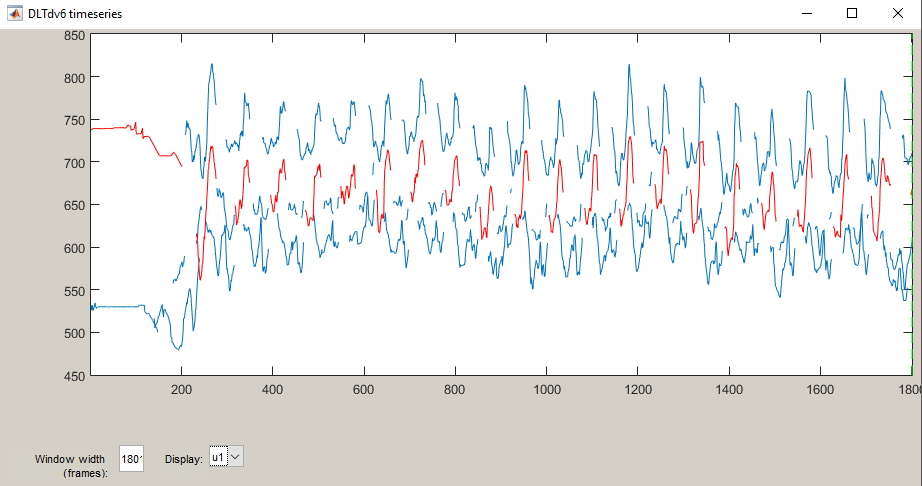
\includegraphics[width=0.5\linewidth]{figures/ipdatapattern.png}
\caption{iamge processing things}
\label{fig:ipdatapattern}
\end{figure}

data successfully captured



\subsection{EFK Results}

see appendix b for availability graphs



\section{Discussion}

THe general system was a successful proof of concept

model was

\subsection{System Modelling}
model was usable and back up by literature review.

The system model had 2 major shortcomings. Firstly the assumption of a rigid chest and secondly the assumption that the cameras stay aligned with the body frame.

It is clear from the Gyroscope data that the chest of a runner oscillates. Since the cameras protrude from the chest they move in an arc pattern in space. 

The model proved sufficient

talk about how the model would also allow the sensor to be used for subjects with prosthesis and allow for better understanding of disabled persons.

\subsection{Image Processing}
THe techniques of image processing considered in this thesis shows the difficulty in implementing an automated image processing system.

\subsection{Extended Kalman Filter}
The filter had limited results












